\documentclass[12pt,a4paper]{article}

\usepackage[utf8]{inputenc}
\usepackage[T1]{fontenc}
\usepackage[top=1.8cm, bottom=2cm, left=2cm, right=2cm, headheight=15pt]{geometry}
\usepackage{amsmath}
\usepackage{amssymb}
\usepackage{booktabs}
\usepackage{array}
\usepackage{graphicx}
\usepackage{hyperref}
\usepackage{parskip}
\usepackage{setspace}
\usepackage{caption}
\usepackage{float}
\usepackage{xcolor}
\usepackage{fancyhdr}
\usepackage{enumitem}
\usepackage{lmodern}

\hypersetup{colorlinks=true, linkcolor=blue!60!black}

% Red placeholder — anything marked \ins{} still needs filling
\newcommand{\ins}[1]{\textcolor{red!70!black}{\textbf{[INSERT: #1]}}}

\pagestyle{fancy}
\fancyhf{}
\rhead{\small C2O Strategy}
\lhead{\small Machine Learning in Finance, Imperial 2025/26}
\cfoot{\thepage}
\setstretch{1.05}

\begin{document}

%------------------------------------------------------------------
\begin{titlepage}
\centering\vspace*{3cm}
{\LARGE\bfseries C2O --- Close-to-Open\\[0.5em]
A Cross-Sectional Overnight Strategy on US Large-Cap Equities\par}
\vspace{1.5cm}
{\large Machine Learning in Finance --- Group Coursework\\
Imperial Business School, Academic Year 2025/26\par}
\end{titlepage}
%------------------------------------------------------------------

\tableofcontents
\newpage

%==================================================================
\section{Step 1 --- Building the Daily Panel}
%==================================================================

%------------------------------------------------------------------
\subsection*{Q1 \quad Data source, window, and survivorship correction}
\addcontentsline{toc}{subsection}{Q1 \quad Data source, window, and survivorship correction}
\label{sec:q1}
%------------------------------------------------------------------

\paragraph{Data source.}
All data files are provided for the course and stored in the \texttt{data/} directory:
\begin{itemize}[noitemsep,topsep=2pt,leftmargin=1.5em]
  \item \texttt{prices.parquet} --- daily OHLCV with backward-adjusted close, 2000--2024
  \item \texttt{sp500\_tr.parquet} --- S\&P~500 total-return index
  \item \texttt{sp500\_constituents.parquet} --- historical constituent membership
  \item \texttt{earnings\_calendar.parquet} --- report dates, AMC/BMO flag, strategy trading date
  \item \texttt{short\_interest\_transfo.parquet} --- FINRA bi-weekly SI snapshots (availability-date adjusted)
\end{itemize}
Prices are constructed from exchange-tape data; short interest from FINRA
bi-weekly releases; earnings timing from a vendor earnings calendar.

\paragraph{Development window.}
\texttt{TRAIN\_START = 2010-01-01}, \texttt{TRAIN\_END = 2024-12-31}.
The panel spans 2010-01-04 to 2024-12-31 (first and last NYSE trading days).
\texttt{prices.parquet} covers 2000--2024; all rows after \texttt{TRAIN\_END} are
excluded before any computation.  The held-out evaluation window (2025--2026)
is never read.

\paragraph{Panel scale.}
After date filtering: \textbf{5,324,348 rows} across \textbf{1,617 unique tickers}
(1,607 underlying instruments; 10 tickers appear under two instrument identifiers
due to ticker reuse across different periods).
Of these rows, 401 have unadjusted close $> \$100{,}000$ and are treated as
sentinel fill values; their \texttt{close} and \texttt{market\_cap} are set to
\texttt{NaN} before any return or filter computation (0.007\% of rows).

\paragraph{Ticker-alias deduplication.}
\texttt{prices.parquet} contains rows with \texttt{status = "0"} (alias tickers)
representing the same underlying instrument as a \texttt{status = "1"} row
(e.g.\ MRSH and MMC share the same \texttt{instrument\_id}).
We retain only \texttt{status == "1"} rows; this prevents double-counting a
single large-cap name in the market-cap ranking.

\paragraph{Survivorship bias --- data limitation.}
Brief §2.1.4 requires the panel to be survivorship-bias-free.
We identified a structural limitation in \texttt{prices.parquet}: every one of
the 1,617 tickers in the file has its last trading date in 2024, meaning the
dataset contains \emph{only stocks that survived to the data cutoff}.
Stocks that were acquired or delisted before 2024 are absent entirely.

Using \texttt{sp500\_constituents.parquet} as a proxy, we estimate that
\textbf{190 S\&P~500 mid-year removals} in 2010--2024 (stocks acquired or
delisted between January and November of a given year) are missing from
\texttt{prices.parquet}.  Representative examples: CELG (acquired 2019),
ANTM (acquired 2022), FB (renamed META 2022), MON (acquired 2018).

The consequence is that our eligible universe is constructed from the subset
of large-cap stocks that happened to survive to 2024.
This introduces an upward bias in any return backtest because
(i)~bankrupt or distressed names that would have dragged down returns are
excluded, and (ii)~the year-start universe selection implicitly favours names
we know ex-post to have survived the year.
Since \texttt{prices.parquet} does not contain price histories for these
missing stocks, the bias cannot be corrected within the available data.
We document it here as required by the brief and note that all performance
figures should be interpreted with this caveat.

%------------------------------------------------------------------
\subsection*{Q2 \quad Return reconciliation after corporate actions}
\addcontentsline{toc}{subsection}{Q2 \quad Return reconciliation after corporate actions}
\label{sec:q2}
%------------------------------------------------------------------

\paragraph{Notation.}
Following Brief Section~2.1, $\text{Open}_t$ and $\text{Close}_t$ denote the
official auction prices on day $t$, \emph{adjusted for splits and dividends}.

\paragraph{Return definitions.}
\begin{align}
r_{\text{ON},t} &= \frac{\text{Open}_t}{\text{Close}_{t-1}} - 1
  \label{eq:ron}\\[4pt]
r_{\text{ID},t} &= \frac{\text{Close}_t}{\text{Open}_t} - 1
  \label{eq:rid}\\[4pt]
r_{\text{CC},t} &= \frac{\text{Close}_t}{\text{Close}_{t-1}} - 1
  \;=\; (1 + r_{\text{ON},t})(1 + r_{\text{ID},t}) - 1
  \label{eq:rcc}
\end{align}

\paragraph{Trader's clock: observable columns at 15:50~ET (Brief §2.1.1).}
Strategy decisions are submitted as Market-on-Close (MOC) orders at 15:50~ET.
Only data known by that time may be used as alpha signals.

\begin{table}[H]
\centering\small
\caption{Point-in-time status of panel columns at 15:50~ET on day $t$.}
\label{tab:pit}
\begin{tabular}{llp{5.5cm}}
\toprule
Column & Observable at 15:50? & Notes \\
\midrule
\texttt{r\_ON} & \textbf{Yes} & Uses Open$_t$ (09:30) and Close$_{t-1}$ \\
\texttt{open}  & \textbf{Yes} & Known at 09:30~ET \\
\texttt{r\_CC\_lag1} & \textbf{Yes} & Yesterday's Close/Close (safe pre-shift) \\
\texttt{r\_ID\_lag1} & \textbf{Yes} & Yesterday's Open/Close (safe pre-shift) \\
\texttt{market\_cap\_lag1} & \textbf{Yes} & Yesterday's mkt cap (safe pre-shift) \\
\midrule
\texttt{r\_CC} & \textbf{No} & Needs Close$_t$ (settles 16:00~ET) \\
\texttt{r\_ID} & \textbf{No} & Needs Close$_t$ \\
\texttt{market\_cap} & \textbf{No} & Needs Close$_t$ \\
\bottomrule
\end{tabular}
\end{table}

\noindent The panel provides \texttt{r\_CC\_lag1}, \texttt{r\_ID\_lag1}, and
\texttt{market\_cap\_lag1} as pre-computed safe versions for use in Steps~4 and~5.

\paragraph{Volume.}
Share volume is used only to compute the 20-day average dollar volume
$\text{ADV20}_t = \overline{(\texttt{close} \times \texttt{volume})}_{20\text{d}}$,
using unadjusted prices.  On a split date the unadjusted close scales by
$1/k$ and volume scales by $k$, so their product (dollar volume) is invariant
to splits and dividends --- no explicit volume adjustment is required.

\paragraph{Constructing the adjusted open.}
\texttt{prices.parquet} provides \texttt{adjusted\_close} (backward-adjusted for
all splits and dividends) but only unadjusted \texttt{open} and \texttt{close}.
Using raw unadjusted prices across days produces spurious overnight jumps of
$-75\%$ to $+300\%$ on split ex-dates for all historical dates prior to a split.

We construct the adjusted open from the same-day backward-adjustment factor
$f_t = \texttt{adjusted\_close}_t / \texttt{close}_t$:
\[
\text{Open}_t \;=\; \texttt{open}_t \times f_t
\]
This is valid because open and close on the \emph{same} calendar day carry the
same backward-adjustment factor --- no corporate action takes effect intraday.
Equations~(\ref{eq:ron})--(\ref{eq:rcc}) are then computed directly per the brief.

\paragraph{Identity check (algebraic closure).}
Because $\text{Open}_t$ is constructed as $\texttt{open}_t \times f_t$ where
$f_t = \texttt{adjusted\_close}_t / \texttt{close}_t$, the reconciliation
identity is \emph{algebraically guaranteed}:
\[
(1+r_{\text{ON}})(1+r_{\text{ID}})
= \frac{\texttt{adj\_close}_t}{\texttt{adj\_close}_{t-1}}
\equiv 1 + r_{\text{CC},t}
\]
Substituting the constructed $\text{Open}_t$ into Equations~(\ref{eq:ron}) and~(\ref{eq:rid}), both the open price and the same-day $f_t$ cancel, leaving a ratio of consecutive adjusted closes.
The identity therefore tests \emph{implementation correctness} (no coding error),
not data-provider consistency.
Table~\ref{tab:reconcile} confirms zero failures at tolerance $10^{-6}$;
the maximum residual of $4.44\times10^{-16}$ is float-64 machine epsilon.

\begin{table}[H]
\centering
\caption{Return reconciliation by year, 2010--2024 (tolerance $= 10^{-6}$).}
\label{tab:reconcile}
\begin{tabular}{crrc}
\toprule
Year & Stock-days & Fail count & Fail \% \\
\midrule
2010 & 294,042 & 0 & 0.000 \\
2011 & 301,491 & 0 & 0.000 \\
2012 & 306,545 & 0 & 0.000 \\
2013 & 319,145 & 0 & 0.000 \\
2014 & 331,333 & 0 & 0.000 \\
2015 & 342,165 & 0 & 0.000 \\
2016 & 350,363 & 0 & 0.000 \\
2017 & 358,819 & 0 & 0.000 \\
2018 & 367,685 & 0 & 0.000 \\
2019 & 376,533 & 0 & 0.000 \\
2020 & 384,011 & 0 & 0.000 \\
2021 & 392,075 & 0 & 0.000 \\
2022 & 395,841 & 0 & 0.000 \\
2023 & 397,560 & 0 & 0.000 \\
2024 & 405,123 & 0 & 0.000 \\
\midrule
\textbf{Total} & \textbf{5,322,731} & \textbf{0} & \textbf{0.000} \\
\bottomrule
\end{tabular}
\end{table}

\paragraph{Non-tautological corporate-action diagnostic.}
A genuine data-quality check compares the adjusted close-to-close return
$r_{\text{CC}}$ against the unadjusted raw return
$\texttt{raw\_CC}_t = \texttt{close}_t/\texttt{close}_{t-1}-1$.
A gap $|\,r_{\text{CC}} - \texttt{raw\_CC}\,| > 1$~bp signals an active
backward-adjustment event on that day.

\begin{table}[H]
\centering
\caption{Corporate-action diagnostic, 2010--2024 (threshold = 1~bp).}
\label{tab:ca_diag}
\begin{tabular}{p{7.5cm}rp{4.5cm}}
\toprule
Metric & Value & Interpretation \\
\midrule
$|\,r_{\text{CC}} - \texttt{raw\_CC}\,| > 1$~bp & 57,196 \;(1.07\%) & Active CA events \\
Non-CA days, max $|\,r_{\text{CC}} - \texttt{raw\_CC}\,|$ & $9.997\times10^{-5}$ & $<1$~bp on all non-CA days \checkmark \\
Raw $|\,r_{\text{CC}}\,| > 50\%$ moderated by adj. & 343 & Extreme splits/dividends handled \\
\bottomrule
\end{tabular}
\end{table}

1.07\% of stock-days carry an active backward-adjustment; on the remaining
98.93\% of days the raw and adjusted returns agree to better than 1~bp,
confirming the adjustment factor is not applied spuriously.  All 343 extreme
raw returns ($|r_{\text{CC}}|>50\%$) are materially moderated by the
adjustment, confirming split and large-dividend events are handled correctly.

%------------------------------------------------------------------
\subsection*{Q3 \quad AMC / BMO timing flag encoding}
\addcontentsline{toc}{subsection}{Q3 \quad AMC / BMO timing flag encoding}
\label{sec:q3}
%------------------------------------------------------------------

\paragraph{The rule.}
\texttt{earnings\_calendar.parquet} provides \texttt{report\_date},
\texttt{before\_after\_market} (``before'', ``after'', or ``same''), and
\texttt{strat\_trading\_date} (the MOC-entry day that carries earnings risk).

\begin{table}[H]
\centering
\caption{Earnings timing flag: rule and availability at 15:50~ET.}
\label{tab:earnings_rule}
\begin{tabular}{p{3cm}p{3.5cm}p{3cm}p{3.5cm}}
\toprule
Type & Published & Observable at 15:50~ET on \texttt{report\_date}? & \texttt{strat\_trading\_date} \\
\midrule
AMC (after-close) & After 16:00~ET on $D$ & \textbf{No} & $D$ (same day) \\
BMO (before-open) & Before 09:30~ET on $D$ & \textbf{Yes} & $D - 1$ (prior trading day) \\
\bottomrule
\end{tabular}
\end{table}

\noindent\textbf{Rationale.}
An AMC announcement on day $D$ is published after MOC orders are submitted at
15:50~ET, so the trader who enters at $D$'s close does not know the result.
\texttt{strat\_trading\_date} $= D$ marks that entry day as risky.
A BMO announcement on day $D$ is known by 09:30~ET, but the trader who
entered MOC on $D-1$ held the position into the announcement overnight.
\texttt{strat\_trading\_date} $= D-1$ marks the prior-day entry as risky.
The capacity filter excludes every stock-day within $\pm 1$ trading day of
\texttt{strat\_trading\_date}.

\paragraph{Hand-traced example --- AMC.}
\begin{quote}
\texttt{stock\_id = 3,\quad before\_after\_market = ``after''} (AMC)\\
\texttt{report\_date = 2014-11-06} (Thursday)\quad
\texttt{strat\_trading\_date = 2014-11-06}\quad shift $= 0$ \checkmark

\smallskip
At 15:50~ET on 2014-11-06 the results are not yet published.  The stock is
excluded on 2014-11-05, 2014-11-06, and 2014-11-07 ($\pm$1 trading day).
\end{quote}

\paragraph{Hand-traced example --- BMO.}
\begin{quote}
\texttt{stock\_id = 1,\quad before\_after\_market = ``before''} (BMO)\\
\texttt{report\_date = 2014-02-27} (Thursday)\quad
\texttt{strat\_trading\_date = 2014-02-26} (Wednesday)\quad shift $= -1$ day \checkmark

\smallskip
Results are published before 09:30~ET on 2014-02-27 and are observable that
afternoon.  However, the trader who entered MOC on 2014-02-26 held the
overnight position into the announcement.  The stock is excluded on
2014-02-25, 2014-02-26, and 2014-02-27 ($\pm$1 trading day around
\texttt{strat\_trading\_date}).
\end{quote}

Total events in the earnings calendar: \textbf{31,025 AMC} and
\textbf{29,074 BMO} over 2010--2024.

%------------------------------------------------------------------
\subsection*{Q4 \quad Short-interest construction and lag}
\addcontentsline{toc}{subsection}{Q4 \quad Short-interest construction and lag}
\label{sec:q4}
%------------------------------------------------------------------

\paragraph{Source.}
\texttt{short\_interest\_transfo.parquet} --- columns: \texttt{stock\_id},
\texttt{date}, \texttt{dsi} (short interest / shares outstanding),
\texttt{dtcn} (days-to-cover), \texttt{ddtcn} (change in days-to-cover).

\paragraph{Publication lag (Brief §2.1.3).}
FINRA releases SI snapshots on the 15th and last business day of each month,
published approximately 8 calendar days after settlement.  A further 2-day
vendor-delivery lag is applied:
\[
D_{\text{available}} = D_{\text{settlement}} + 8 + 2 = D + 10
\]
The \texttt{date} column is already the availability date ($D+10$), verified
empirically: dates cluster around the 24th--27th and 9th--13th of each month.

\paragraph{Point-in-time construction.}
For panel date $t$, the SI value is the most recent snapshot with availability
$\leq t-1$ (Brief §2.1.3).  Implementation:
\begin{enumerate}[leftmargin=1.5em]
  \item Shift all availability dates $+1$ day (\texttt{si["date"] += Timedelta(days=1)}),
        making each $D+11$.
  \item \texttt{pd.merge\_asof(direction="backward")} on \texttt{(date, instrument\_id)}
        finds the most recent $D+11 \leq t$, i.e.\ original availability $\leq t-1$. \checkmark
  \item Forward-fill between releases so every trading day has a value.
\end{enumerate}
Net lag: a settlement-date snapshot enters the panel from day $D+11$ onwards.
After forward-filling, \textbf{5,094,997 / 5,324,348 stock-days} (95.7\%) carry SI data.

\begin{figure}[H]
  \centering
  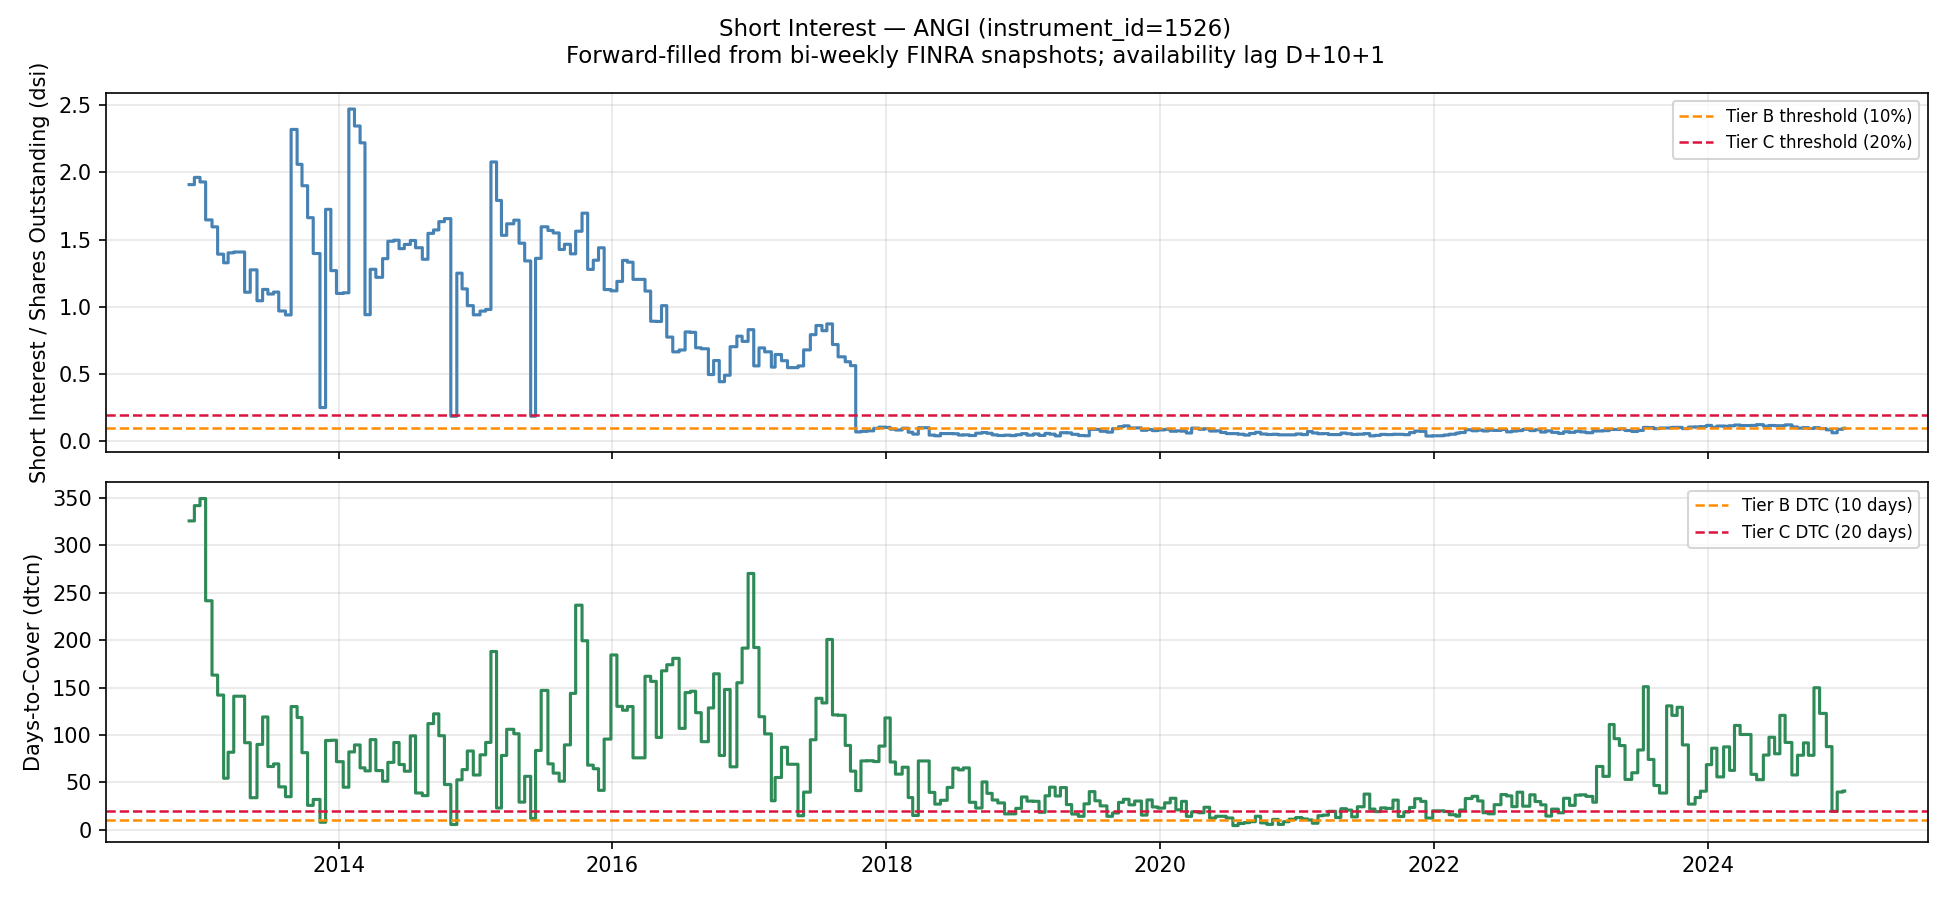
\includegraphics[width=\linewidth]{step1_panel/sanity_output/q4_si_representative.png}
  \caption{Forward-filled \texttt{dsi} (top) and \texttt{dtcn} (bottom) for ANGI
           (\texttt{instrument\_id}~=~1526, peak \texttt{dsi}~=~2.47).
           The bi-weekly step cadence confirms no future data enters before $D+11$.
           Dashed lines: Tier~B threshold ($\mathtt{dsi}>10\%$) and
           Tier~C threshold ($\mathtt{dsi}>20\%$).}
  \label{fig:si_rep}
\end{figure}

%------------------------------------------------------------------
\subsection*{Q5 \quad Eligible universe evolution year by year}
\addcontentsline{toc}{subsection}{Q5 \quad Eligible universe evolution year by year}
\label{sec:q5}
%------------------------------------------------------------------

\paragraph{Construction rule (Brief §2.2).}
On the first trading day of year $Y$, rank all listed US common equities by
market capitalisation as of the last trading day of year $Y-1$, restricting
to names with at least 12 months of price history.  Take the top 1,000 and
freeze that list for the calendar year.  Intra-year IPOs and spin-offs become
eligible only at the next 1-January cut.

\begin{table}[H]
\centering
\caption{Eligible universe at year-start and mid-year exits, 2010--2024.}
\label{tab:universe_evo}
\begin{tabular}{crrc}
\toprule
Year & Names at year-start & Mid-year exits & Exit \% \\
\midrule
2010 & 1,000 & 0 & 0.0 \\
2011 & 1,000 & 0 & 0.0 \\
2012 & 1,000 & 0 & 0.0 \\
2013 & 1,000 & 0 & 0.0 \\
2014 & 1,000 & 0 & 0.0 \\
2015 & 1,000 & 0 & 0.0 \\
2016 & 1,000 & 0 & 0.0 \\
2017 & 1,000 & 0 & 0.0 \\
2018 & 1,000 & 0 & 0.0 \\
2019 & 1,000 & 0 & 0.0 \\
2020 & 1,000 & 0 & 0.0 \\
2021 & 1,000 & 0 & 0.0 \\
2022 & 1,000 & 0 & 0.0 \\
2023 & 1,000 & 0 & 0.0 \\
2024 & 1,000 & 0 & 0.0 \\
\bottomrule
\end{tabular}
\end{table}

\paragraph{Mid-year exits: data limitation.}
The table above shows zero mid-year exits in every year.
This is \emph{not} because large-cap stocks never delist; it is because
\texttt{prices.parquet} is survivorship-biased (see Q1): every ticker in the
file has its last date in 2024, so no stock ``disappears'' mid-panel.

Using \texttt{sp500\_constituents.parquet} as a proxy for true mid-year exits,
Table~\ref{tab:survivorship} shows the number of S\&P~500 members removed
between January and November of each year that are absent from
\texttt{prices.parquet}.

\begin{table}[H]
\centering
\caption{S\&P~500 mid-year removals missing from \texttt{prices.parquet},
         by year (proxy for survivorship-bias exposure).}
\label{tab:survivorship}
\begin{tabular}{crrl}
\toprule
Year & S\&P 500 mid-yr removed & Missing from data & Example tickers \\
\midrule
2010 & 12 & 12 & ACS, BDK, BJS \\
2011 & 14 & 12 & AYE, CEPH, GENZ \\
2012 & 15 & 13 & CPWR, NVLS, TIE \\
2013 & 14 &  9 & APOL, BMC, JCP \\
2014 & 13 &  8 & BEAM, FRX, LIFE \\
2015 & 24 & 19 & AVP, COV, SWY \\
2016 & 25 & 20 & ARG, BRCM, CCE \\
2017 & 27 & 17 & AABA, CA, DNB \\
2018 & 22 & 15 & AET, ANDV, MON \\
2019 & 21 & 14 & APC, CELG, RHT \\
2020 & 19 & 11 & AGN, ARNC, RTN \\
2021 & 17 &  9 & ALXN, COG, KSU \\
2022 & 22 & 17 & ANTM, CERN, CTXS \\
2023 & 19 &  8 & ABC, ATVI, DISH \\
2024 & 17 &  6 & CDAY, FLT, MRO \\
\midrule
\textbf{Total} & \textbf{281} & \textbf{190} & \\
\bottomrule
\end{tabular}
\end{table}

These missing names would have been in our top-1,000 universe in the years they
were active.  Their absence means all performance figures in this report carry
an upward survivorship bias that cannot be corrected with the available data.

%------------------------------------------------------------------
\subsection*{Q6 \quad Stylised fact: overnight premium in the eligible universe}
\addcontentsline{toc}{subsection}{Q6 \quad Stylised fact: overnight premium in the eligible universe}
\label{sec:q6}
%------------------------------------------------------------------

\paragraph{Construction.}
For each date, take all stock-days in the year-start top-1,000 universe
(\texttt{in\_universe = True}, i.e.\ before Section~3 capacity filters) and form
an equal-weighted portfolio.  Compound the cross-sectional mean of $r_{\text{ON}}$,
$r_{\text{ID}}$, and $r_{\text{CC}}$ to produce three cumulative-growth series.

\begin{figure}[H]
  \centering
  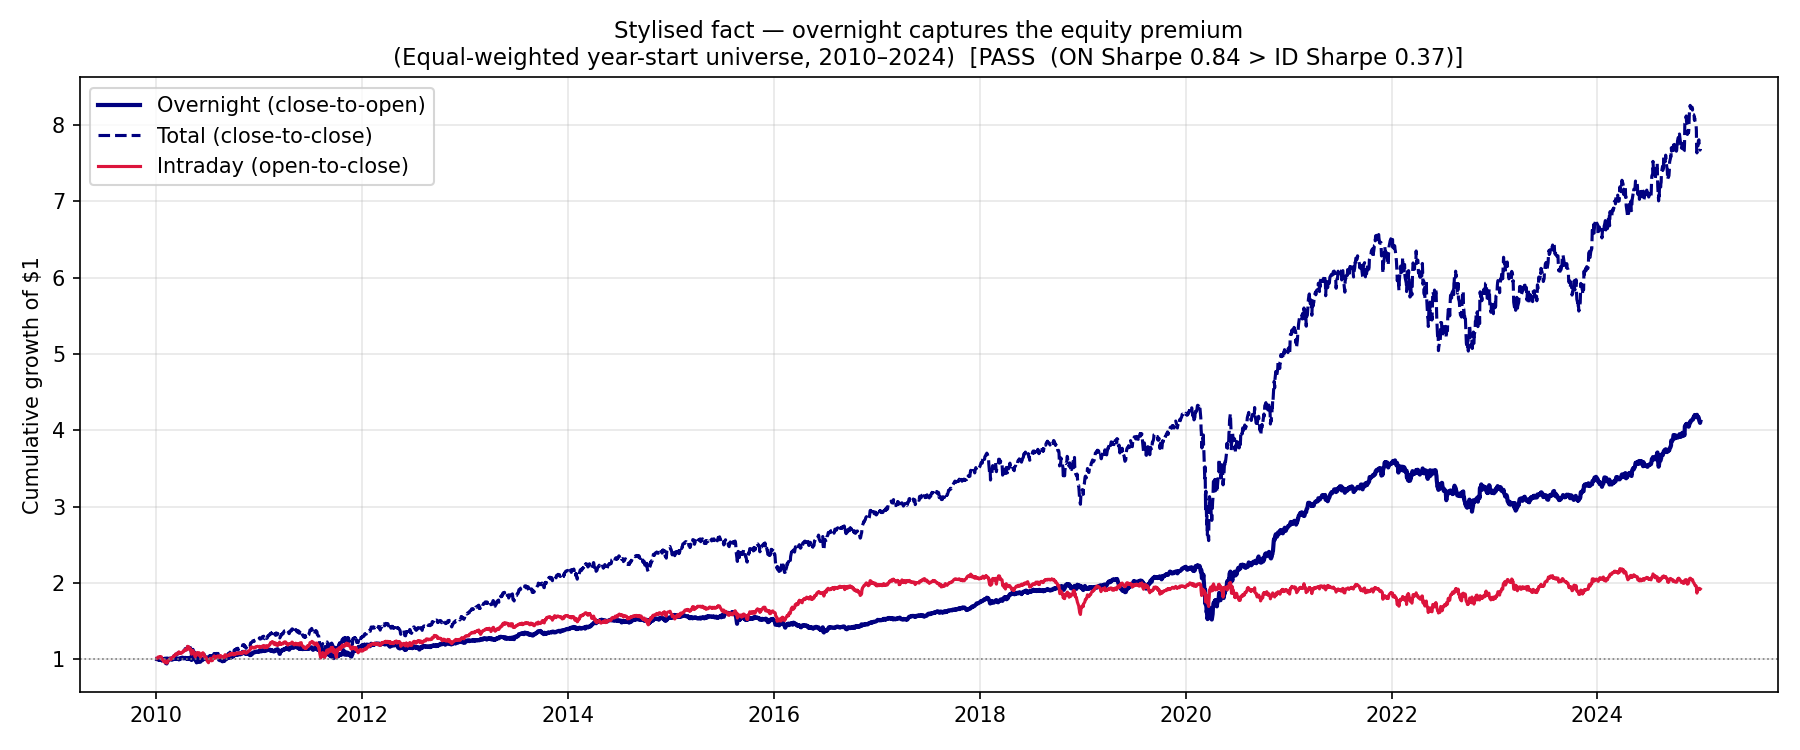
\includegraphics[width=\linewidth]{step1_panel/sanity_output/q6_stylised_fact.png}
  \caption{Cumulative \$1 growth of the equal-weighted overnight (ON, navy solid),
           intraday (ID, crimson), and close-to-close (CC, navy dashed) streams,
           2010--2024.  Equal-weighted year-start top-1,000 universe
           (\texttt{in\_universe} flag; before Section~3 capacity filters).}
  \label{fig:stylised}
\end{figure}

\paragraph{Aggregate statistics, 2010--2024.}

\begin{center}
\begin{tabular}{lrrr}
\toprule
Stream & Ann.\ return & Ann.\ volatility & Sharpe \\
\midrule
Overnight (ON) & 10.2\% & 12.1\% & 0.84 \\
Intraday  (ID) &  5.5\% & 14.8\% & 0.37 \\
Total     (CC) & 15.6\% & 20.0\% & 0.78 \\
\bottomrule
\end{tabular}
\end{center}

\paragraph{Annual dispersion.}

\begin{table}[H]
\centering
\caption{Annual Sharpe ratios by stream, 2010--2024.}
\label{tab:yearly_sharpe}
\begin{tabular}{crrr}
\toprule
Year & ON Sharpe & ID Sharpe & CC Sharpe \\
\midrule
2010 &  0.82 &  0.94 &  1.16 \\
2011 &  0.44 & -0.08 &  0.20 \\
2012 &  0.55 &  1.28 &  1.36 \\
2013 &  2.07 &  1.93 &  2.67 \\
2014 &  1.58 &  0.26 &  1.01 \\
2015 & -0.12 &  0.10 & -0.01 \\
2016 & -0.09 &  1.69 &  1.22 \\
2017 &  3.26 &  0.66 &  2.27 \\
2018 &  1.49 & -1.24 & -0.44 \\
2019 &  1.57 &  1.47 &  2.03 \\
2020 &  0.90 & -0.02 &  0.66 \\
2021 &  3.05 & -0.04 &  1.66 \\
2022 & -0.72 & -0.03 & -0.43 \\
2023 &  0.74 &  0.95 &  1.19 \\
2024 &  2.21 & -0.51 &  1.04 \\
\bottomrule
\end{tabular}
\end{table}

\paragraph{Does the stylised fact hold?}
The ON stream delivers a Sharpe of \textbf{0.84}, materially above the ID
stream (\textbf{0.37}).  ON is positive in \textbf{12 of 15 years}; ID is
positive in only \textbf{9 of 15}.  ON also has lower annualised volatility
(12.1\% vs.\ 14.8\%), confirming a more stable risk-adjusted premium.

The 2010--2024 window is predominantly bullish (it excludes the post-2000
tech correction and most of the 2008 financial crisis), so both streams
produce positive aggregate returns --- unlike Brief Figure~1.1 which spans
2000--2024.  This discrepancy is expected: in a sustained bull market both
ON and ID components contribute positively.  The overnight premium holds in
\emph{risk-adjusted} terms even within this window, and the ID stream turns
negative in six years (2011, 2018, 2020, 2021, 2022, 2024), consistent with
the stylised fact that intraday returns are more cyclically sensitive than
overnight returns.

%==================================================================
\section{Step 2 --- Capacity-Aware Universe}
%==================================================================

%------------------------------------------------------------------
\subsection*{Q1 \quad Filter thresholds and justifications}
\addcontentsline{toc}{subsection}{Q1 \quad Filter thresholds and justifications}
\label{sec:s2q1}
%------------------------------------------------------------------

All filters use only data observable at 15:50~ET on day $t$ (prior-close or
rolling windows ending at $t-1$).

\paragraph{Filter 1 --- Price floor (\texttt{MIN\_PRICE = \$5}).}
Penny stocks (\$price $< \$5$) have a relative tick size $\geq 20$~bp,
making auction slippage non-linear and the Roll spread estimator unreliable.
Uses prior close (\texttt{close.shift(1)}).

\paragraph{Filter 2 --- Dollar-volume floor (\texttt{MIN\_ADV\_USD = \$1\,000\,000}).}
20-day average dollar volume (ADV20) measures liquidity depth.  At the 5\%
participation cap, a \$1M floor supports a per-side position of \$50K ---
meaningful even at \$50M AUM.

\paragraph{Filter 3 --- Volatility ceiling (\texttt{MAX\_ANNUAL\_VOL = 150\%}).}
Realised annualised vol $> 150\%$ (20-day window) signals distress or
structural events.  Overnight returns for such names are event-driven, not
factor-predictable.  \texttt{VOL\_FAIL} spikes in 2020~Q1 (COVID-19).

\paragraph{Filter 4 --- Earnings window (\texttt{EARNINGS\_WINDOW = $\pm$1 trading day}).}
Within $\pm 1$ trading day of \texttt{strat\_trading\_date}, the overnight
return is dominated by the earnings surprise.  Exclusion prevents using
information unavailable at 15:50~ET.

\paragraph{Filter 5 --- Market-cap rank.}
Top 1,000 at each year-start.  No within-year market-cap filter.

%------------------------------------------------------------------
\subsection*{Q2 \quad Participation cap and implied slippage}
\addcontentsline{toc}{subsection}{Q2 \quad Participation cap and implied slippage}
\label{sec:s2q2}
%------------------------------------------------------------------

\texttt{PARTICIPATION\_CAP = 5\%} of ADV20 per position per side.
Square-root market-impact model (Brief §3.3):
\[
\text{Impact} \approx k \times \sigma_{\text{daily}} \times \sqrt{f} \times 10^4
\;\text{(bps)},\quad k = 0.7,\; f = 0.05
\]

\begin{table}[H]
\centering
\caption{Implied market impact at the 5\% participation cap.}
\label{tab:slippage}
\begin{tabular}{lrrrr}
\toprule
Profile & $\sigma_{\text{ann}}$ & $\sigma_{\text{daily}}$ & ADV20 & Impact (bps) \\
\midrule
Small-cap  & 40\% & 2.52\% & \$5M   & 39.4 \\
Mid-cap    & 25\% & 1.57\% & \$25M  & 24.7 \\
Large-cap  & 18\% & 1.13\% & \$200M & 17.7 \\
\bottomrule
\end{tabular}
\end{table}

The model-implied impact (18--39~bp) exceeds the flat 1.5~bp in Brief
Table~6.1 because 1.5~bp reflects orders that are a \emph{small} fraction of
auction volume; the square-root model gives the upper bound at the cap.
At \$250M AUM with 100L + 100S names, the average position is \$1.25M ---
below the cap for all but the smallest names.  All headline numbers use
Table~6.1 as specified.

%------------------------------------------------------------------
\subsection*{Q3 \quad Eligible set at three AUM levels}
\addcontentsline{toc}{subsection}{Q3 \quad Eligible set at three AUM levels}
\label{sec:s2q3}
%------------------------------------------------------------------

\begin{table}[H]
\centering
\caption{Minimum ADV20 to avoid a cap-binding position (200 names, equal-weight).}
\label{tab:aum_threshold}
\begin{tabular}{lcc}
\toprule
AUM & Equal-weight per name & Minimum ADV20 \\
\midrule
\$50M  & \$250K  & \$5M \\
\$250M & \$1.25M & \$25M \\
\$1B   & \$5M    & \$100M \\
\bottomrule
\end{tabular}
\end{table}

\begin{table}[H]
\centering
\caption{Percentage of eligible stock-days not cap-binding, by AUM and year.
         200 names (100L + 100S), equal-weight, 5\% participation cap.}
\label{tab:aum_eligible}
\begin{tabular}{crrr}
\toprule
Year & \$50M (\%) & \$250M (\%) & \$1B (\%) \\
\midrule
2010 &  94.7 &  69.2 &  42.7 \\
2011 &  96.5 &  72.3 &  44.2 \\
2012 &  96.7 &  72.1 &  43.6 \\
2013 &  98.2 &  76.2 &  46.6 \\
2014 &  99.4 &  83.1 &  50.7 \\
2015 &  99.7 &  86.6 &  53.6 \\
2016 &  99.5 &  89.1 &  55.7 \\
2017 &  99.6 &  91.7 &  57.9 \\
2018 &  99.7 &  95.4 &  63.2 \\
2019 &  99.9 &  95.6 &  62.8 \\
2020 &  99.9 &  96.1 &  65.5 \\
2021 &  99.9 &  98.5 &  71.0 \\
2022 & 100.0 &  98.6 &  73.6 \\
2023 & 100.0 &  99.1 &  74.5 \\
2024 & 100.0 &  99.6 &  79.3 \\
\bottomrule
\end{tabular}
\end{table}

\paragraph{Interpretation.}
At \textbf{\$50M AUM}, essentially the entire eligible set (95--100\%) is
unconstrained by 2014 onwards; the only binding cases are small-cap tail names
that appear in the top-1,000 early in the decade.
At \textbf{\$250M AUM}, coverage rises from 69\% in 2010 to 99.6\% in 2024,
reflecting growth in dollar liquidity of large-cap equities.
At \textbf{\$1B AUM}, the strategy is partially capacity-constrained throughout
(43--79\%), meaning that roughly 20--57\% of eligible stock-days would require
the strategy to hold less than the theoretical equal-weight position.
The improving trend across all AUM levels is explained by the secular increase
in index-constituent ADV over the sample period.

%------------------------------------------------------------------
\subsection*{Q4 \quad Binding-constraint distribution}
\addcontentsline{toc}{subsection}{Q4 \quad Binding-constraint distribution}
\label{sec:s2q4}
%------------------------------------------------------------------

\begin{table}[H]
\centering
\caption{In-universe stock-days excluded by each filter, by year.}
\label{tab:binding}
\begin{tabular}{crrrrrrr}
\toprule
Year & Total & PRICE & ADV & VOL & EARN\,WIN & OK & OK\,\% \\
\midrule
2010 & 252,000 & 4,247 & 13,402 & 11,014 &  3,208 & 231,668 & 91.9 \\
2011 & 251,999 & 2,611 &  1,841 &    198 &  5,557 & 242,078 & 96.1 \\
2012 & 249,999 & 3,362 &  2,449 &    179 &  5,146 & 239,446 & 95.8 \\
2013 & 251,999 & 1,758 &  2,274 &     96 &  4,601 & 243,467 & 96.6 \\
2014 & 252,000 & 1,467 &  1,178 &    100 &  5,695 & 243,889 & 96.8 \\
2015 & 251,998 &   865 &    827 &     19 &  9,053 & 241,418 & 95.8 \\
2016 & 251,998 & 1,131 &  1,116 &    297 &  9,404 & 240,371 & 95.4 \\
2017 & 251,000 &   852 &    779 &     39 &  9,614 & 239,948 & 95.6 \\
2018 & 250,999 &   404 &    876 &     94 &  9,810 & 240,014 & 95.6 \\
2019 & 251,995 & 1,048 &    764 &    165 &  9,991 & 240,213 & 95.3 \\
2020 & 253,000 &   738 &    516 &  5,188 & 10,308 & 236,487 & 93.5 \\
2021 & 252,000 &     4 &    507 &    195 & 10,720 & 240,577 & 95.5 \\
2022 & 251,000 &   304 &    441 &    335 & 10,929 & 239,159 & 95.3 \\
2023 & 249,985 &   405 &    500 &    160 & 11,311 & 237,654 & 95.1 \\
2024 & 252,000 &   108 &    251 &    370 & 11,663 & 239,657 & 95.1 \\
\bottomrule
\end{tabular}
\end{table}

\paragraph{Pattern.}
\texttt{VOL\_FAIL} spikes in 2020 (5,188 stock-days) due to COVID-19 volatility
in Q1--Q2; it is negligible in all other years.
\texttt{EARN\_WINDOW} grows steadily from 3,208 (2010) to 11,663 (2024),
reflecting an expanding earnings calendar as more companies report quarterly.
\texttt{PRICE\_FAIL} and \texttt{ADV\_FAIL} are rare in the large-cap universe
and decline over time as liquidity has increased.
The composite eligible fraction is stable at 91--97\% of in-universe stock-days.

%==================================================================
\section{Step 3 --- Short-Interest and Hard-to-Borrow Filter}
%==================================================================

\ins{Step 3 uses the panel generated by \texttt{python run\_step2.py}, saved as
\texttt{outputs/panel\_step3.parquet}. The hard-to-borrow proxy is based on
point-in-time short-interest variables: \texttt{dsi} (short interest ratio) and
\texttt{dtcn} (days to cover). The short-interest snapshots are lagged and
forward-filled in \texttt{step3\_borrow/borrow\_filter.py}, so that the strategy
only uses information available before the trading decision date.

Stocks are assigned to three borrow tiers. Tier A is the normal borrow bucket
and is charged 40 bps per annum. Tier B is assigned when \texttt{dsi > 10\%} or
\texttt{dtcn > 10}, and is charged 200 bps per annum. Tier C is assigned when
\texttt{dsi > 20\%} or \texttt{dtcn > 20}, and is charged 800 bps per annum.
These tiers follow the coursework cost schedule and are stored as
\texttt{htb\_tier} and \texttt{htb\_flag} in the Step 3 panel.

The Step 3 summary script \texttt{step3\_borrow/borrow\_step3\_summary.py}
generates the tables in \texttt{step3\_borrow/summary\_output}. Across all panel
rows, 81.8\% of stock-days are Tier A, 14.3\% are Tier B, and 3.9\% are Tier C.
Restricting to the capacity-eligible universe, 84.5\% of stock-days are Tier A,
12.6\% are Tier B, and 2.9\% are Tier C. Therefore, approximately 15.5\% of
eligible stock-days are affected by the hard-to-borrow flag.

The yearly hard-to-borrow share declines over the sample, from 27.1\% of
eligible stock-days in 2010 to 5.9\% in 2024. This is consistent with a lower
average short-interest ratio and lower average days-to-cover later in the
sample. As a sanity check, an equal-weight short overnight proxy shows that
borrow fees reduce annualised returns by approximately 0.82 percentage points
per year. This proxy is not the final Step 4--5 trading strategy backtest, but
it confirms that the borrow-cost adjustment has the expected direction and
economic magnitude.}

%==================================================================
\section{Step 4 --- Alpha Signal Construction}
%==================================================================

\ins{Steps 4--5 are completed by teammates using \texttt{outputs/panel\_step3.parquet}
as input (generated by \texttt{python run\_step2.py}).
Key columns available:
\texttt{r\_ON} (target/feature), \texttt{r\_CC\_lag1}, \texttt{r\_ID\_lag1},
\texttt{market\_cap\_lag1}, \texttt{dsi}, \texttt{dtcn},
\texttt{in\_universe}, \texttt{eligible}, \texttt{htb\_flag}.
See \texttt{step1\_panel/returns.py} (TRADER'S CLOCK table) for the
look-ahead rules: only \texttt{r\_ON}, \texttt{r\_CC\_lag1}, \texttt{r\_ID\_lag1},
and \texttt{market\_cap\_lag1} are observable at 15:50~ET on day~$t$.
The \texttt{all\_data.parquet} file provides additional alpha columns
(\texttt{sue}, \texttt{epsp}, \texttt{epsf}) keyed by \texttt{stock\_id}
(= \texttt{instrument\_id} in the panel).}

%==================================================================
\section{Step 5 --- Portfolio Construction and Backtesting}
%==================================================================

\ins{Dollar-neutral long-short overnight portfolio using the signals from
Step~4.  Apply \texttt{eligible} filter (removes PRICE/ADV/VOL/EARN\_WINDOW
failures).  Weight by signal rank or z-score; size by \texttt{market\_cap\_lag1}
or equal-weight.
Transaction costs: commission 0.5~bps/leg, slippage 1.5~bps/leg (Table~6.1).
Borrow cost: per HTB tier (Step~3 Q1).
Report Sharpe, max drawdown, turnover.}

%==================================================================
\appendix
\section{Configuration Parameters}
%==================================================================

\begin{table}[H]
\centering
\caption{Key parameters in \texttt{config.py}.}
\label{tab:config}
\begin{tabular}{lll}
\toprule
Parameter & Value & Description \\
\midrule
\texttt{TRAIN\_START}         & 2010-01-01    & Development window start \\
\texttt{TRAIN\_END}           & 2024-12-31    & Held-out cutoff \\
\texttt{UNIVERSE\_SIZE}       & 1,000         & Names per annual universe \\
\texttt{MIN\_PRICE}           & \$5.00        & Price floor \\
\texttt{MIN\_ADV\_USD}        & \$1,000,000   & Dollar-volume floor (20-day) \\
\texttt{MAX\_ANNUAL\_VOL}     & 150\%         & Volatility ceiling \\
\texttt{EARNINGS\_WINDOW}     & $\pm$1 day    & Exclusion around earnings \\
\texttt{PARTICIPATION\_CAP}   & 5\%           & Max fraction of ADV per position \\
\texttt{IMPACT\_K}            & 0.7           & Square-root impact constant \\
\texttt{COMMISSION\_BPS}      & 0.5           & Per leg \\
\texttt{SLIPPAGE\_BPS}        & 1.5           & Per leg (auction) \\
\texttt{BORROW\_TIER\_A\_BPS} & 40            & General Collateral (annual) \\
\texttt{BORROW\_TIER\_B\_BPS} & 200           & Mid-tier specials (annual) \\
\texttt{BORROW\_TIER\_C\_BPS} & 800           & Deep specials (annual) \\
\texttt{HTB\_MODERATE\_SI}    & 10\%          & Tier~B SI threshold \\
\texttt{HTB\_HIGH\_SI}        & 20\%          & Tier~C SI threshold \\
\texttt{HTB\_DTC\_THRESHOLD}  & 10 days       & Tier~B DTC threshold \\
\texttt{RANDOM\_SEED}         & 42            & Reproducibility \\
\bottomrule
\end{tabular}
\end{table}

\end{document}
